\documentclass{standalone}
\usepackage{tikz}
\usetikzlibrary{patterns, positioning}
\usepackage[sfdefault]{ClearSans} %% option 'sfdefault' activates Clear Sans as the default text font
\usepackage[T1]{fontenc}

\begin{document}
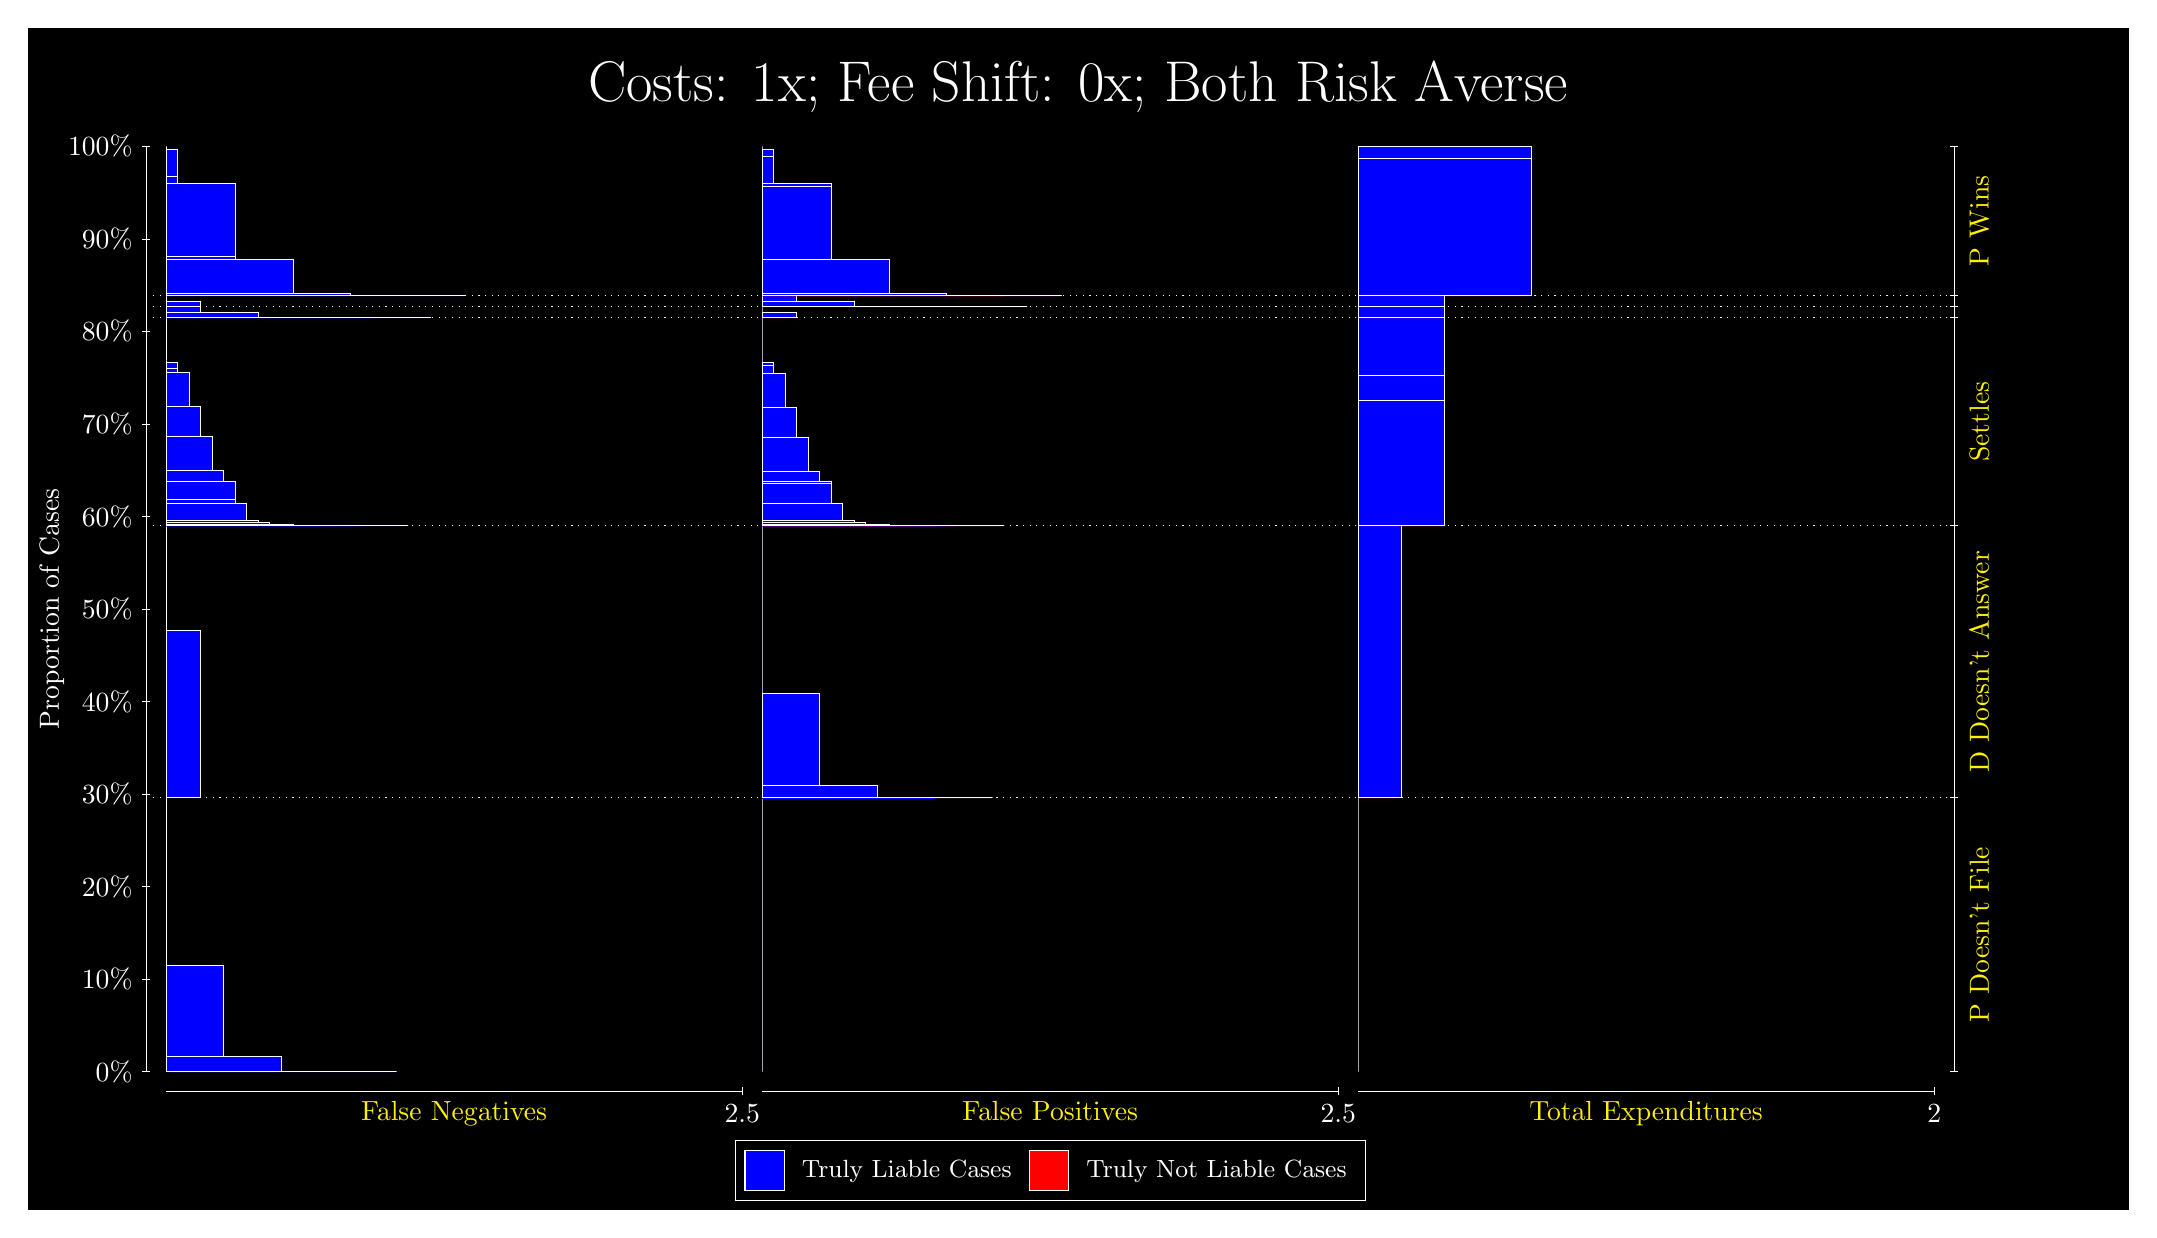
\begin{tikzpicture}
\draw[fill=black] (0,0) rectangle (26.667,15);
\draw[text=white] (0,13.5) rectangle (26.667,15) node[midway] {\huge Costs: 1x; Fee Shift: 0x; Both Risk Averse};
\draw[white, very thin] (1.5,1.75) -- (1.5,13.5);
\node[rotate=90, text=white, anchor=center] at (0.3, 7.625) {Proportion of Cases};
\draw[white, very thin] (1.45,1.75) -- (1.55,1.75);
\node[text=white, anchor=east] at (1.45, 1.75) {0\%};
\draw[white, very thin] (1.45,2.925) -- (1.55,2.925);
\node[text=white, anchor=east] at (1.45, 2.925) {10\%};
\draw[white, very thin] (1.45,4.1) -- (1.55,4.1);
\node[text=white, anchor=east] at (1.45, 4.1) {20\%};
\draw[white, very thin] (1.45,5.275) -- (1.55,5.275);
\node[text=white, anchor=east] at (1.45, 5.275) {30\%};
\draw[white, very thin] (1.45,6.45) -- (1.55,6.45);
\node[text=white, anchor=east] at (1.45, 6.45) {40\%};
\draw[white, very thin] (1.45,7.625) -- (1.55,7.625);
\node[text=white, anchor=east] at (1.45, 7.625) {50\%};
\draw[white, very thin] (1.45,8.8) -- (1.55,8.8);
\node[text=white, anchor=east] at (1.45, 8.8) {60\%};
\draw[white, very thin] (1.45,9.975) -- (1.55,9.975);
\node[text=white, anchor=east] at (1.45, 9.975) {70\%};
\draw[white, very thin] (1.45,11.15) -- (1.55,11.15);
\node[text=white, anchor=east] at (1.45, 11.15) {80\%};
\draw[white, very thin] (1.45,12.325) -- (1.55,12.325);
\node[text=white, anchor=east] at (1.45, 12.325) {90\%};
\draw[white, very thin] (1.45,13.5) -- (1.55,13.5);
\node[text=white, anchor=east] at (1.45, 13.5) {100\%};

\draw[white, very thin] (24.457,1.75) -- (24.457,13.5);
\draw[white, very thin] (24.407,1.75) -- (24.507,1.75);
\node[anchor=west] at (24.407, 1.75) {};
\draw[white, very thin] (24.407,5.2269) -- (24.507,5.2269);
\node[anchor=west] at (24.407, 5.2269) {};
\draw[white, very thin] (24.407,8.6811) -- (24.507,8.6811);
\node[anchor=west] at (24.407, 8.6811) {};
\draw[white, very thin] (24.407,11.325) -- (24.507,11.325);
\node[anchor=west] at (24.407, 11.325) {};
\draw[white, very thin] (24.407,11.465) -- (24.507,11.465);
\node[anchor=west] at (24.407, 11.465) {};
\draw[white, very thin] (24.407,11.605) -- (24.507,11.605);
\node[anchor=west] at (24.407, 11.605) {};
\draw[white, very thin] (24.407,13.5) -- (24.507,13.5);
\node[anchor=west] at (24.407, 13.5) {};

\draw[white, very thin, fill=blue] (1.75,1.75) rectangle (4.6775,1.75);
\draw[white, very thin, fill=blue] (1.75,1.75) rectangle (3.9457,1.7516);
\draw[white, very thin, fill=blue] (1.75,1.7516) rectangle (3.2138,1.9377);
\draw[white, very thin, fill=blue] (1.75,1.9377) rectangle (2.4819,3.1027);
\draw[white, very thin, fill=red] (1.75,3.1027) rectangle (1.75,3.1027);
\draw[white, very thin, fill=blue] (1.75,3.1027) rectangle (1.75,5.2269);
\draw[white, very thin, fill=blue] (1.75,5.2269) rectangle (2.1891,7.3515);
\draw[white, very thin, fill=red] (1.75,7.3515) rectangle (1.75,7.3515);
\draw[white, very thin, fill=blue] (1.75,7.3515) rectangle (1.75,8.6811);
\draw[white, very thin, fill=blue] (1.75,8.6811) rectangle (4.8239,8.6811);
\draw[white, very thin, fill=blue] (1.75,8.6811) rectangle (4.2384,8.6811);
\draw[white, very thin, fill=blue] (1.75,8.6811) rectangle (4.092,8.6811);
\draw[white, very thin, fill=blue] (1.75,8.6811) rectangle (3.9457,8.6811);
\draw[white, very thin, fill=blue] (1.75,8.6811) rectangle (3.6529,8.6811);
\draw[white, very thin, fill=blue] (1.75,8.6811) rectangle (3.5065,8.687);
\draw[white, very thin, fill=blue] (1.75,8.687) rectangle (3.3602,8.6999);
\draw[white, very thin, fill=blue] (1.75,8.6999) rectangle (3.2138,8.7003);
\draw[white, very thin, fill=blue] (1.75,8.7003) rectangle (3.0674,8.7253);
\draw[white, very thin, fill=blue] (1.75,8.7253) rectangle (2.921,8.7506);
\draw[white, very thin, fill=blue] (1.75,8.7506) rectangle (2.7746,8.9725);
\draw[white, very thin, fill=blue] (1.75,8.9725) rectangle (2.6283,9.0224);
\draw[white, very thin, fill=blue] (1.75,9.0224) rectangle (2.6283,9.2524);
\draw[white, very thin, fill=blue] (1.75,9.2524) rectangle (2.4819,9.3839);
\draw[white, very thin, fill=blue] (1.75,9.3839) rectangle (2.3355,9.8174);
\draw[white, very thin, fill=blue] (1.75,9.8174) rectangle (2.1891,10.199);
\draw[white, very thin, fill=blue] (1.75,10.199) rectangle (2.0428,10.629);
\draw[white, very thin, fill=blue] (1.75,10.629) rectangle (1.8964,10.687);
\draw[white, very thin, fill=blue] (1.75,10.687) rectangle (1.8964,10.762);
\draw[white, very thin, fill=blue] (1.75,10.762) rectangle (1.75,10.783);
\draw[white, very thin, fill=red] (1.75,10.783) rectangle (1.75,10.783);
\draw[white, very thin, fill=blue] (1.75,10.783) rectangle (1.75,11.325);
\draw[white, very thin, fill=blue] (1.75,11.325) rectangle (5.1167,11.325);
\draw[white, very thin, fill=blue] (1.75,11.325) rectangle (4.3848,11.325);
\draw[white, very thin, fill=blue] (1.75,11.325) rectangle (3.6529,11.327);
\draw[white, very thin, fill=blue] (1.75,11.327) rectangle (2.921,11.398);
\draw[white, very thin, fill=blue] (1.75,11.398) rectangle (2.1891,11.465);
\draw[white, very thin, fill=red] (1.75,11.465) rectangle (1.75,11.465);
\draw[white, very thin, fill=blue] (1.75,11.465) rectangle (2.1891,11.533);
\draw[white, very thin, fill=red] (1.75,11.533) rectangle (1.75,11.533);
\draw[white, very thin, fill=blue] (1.75,11.533) rectangle (1.75,11.605);
\draw[white, very thin, fill=blue] (1.75,11.605) rectangle (5.5558,11.605);
\draw[white, very thin, fill=blue] (1.75,11.605) rectangle (4.8239,11.606);
\draw[white, very thin, fill=blue] (1.75,11.606) rectangle (4.092,11.639);
\draw[white, very thin, fill=blue] (1.75,11.639) rectangle (3.3602,12.07);
\draw[white, very thin, fill=blue] (1.75,12.07) rectangle (2.6283,12.108);
\draw[white, very thin, fill=blue] (1.75,12.108) rectangle (2.6283,13.036);
\draw[white, very thin, fill=blue] (1.75,13.036) rectangle (1.8964,13.123);
\draw[white, very thin, fill=blue] (1.75,13.123) rectangle (1.8964,13.466);
\draw[white, very thin, fill=red] (1.75,13.466) rectangle (1.75,13.466);
\draw[white, very thin, fill=blue] (1.75,13.466) rectangle (1.75,13.5);
\draw[white, very thin, fill=red] (9.3189,1.75) rectangle (9.3189,1.75);
\draw[white, very thin, fill=blue] (9.3189,1.75) rectangle (9.3189,5.2269);
\draw[white, very thin, fill=red] (9.3189,5.2269) rectangle (12.246,5.2269);
\draw[white, very thin, fill=blue] (9.3189,5.2269) rectangle (12.246,5.2269);
\draw[white, very thin, fill=blue] (9.3189,5.2269) rectangle (11.515,5.2274);
\draw[white, very thin, fill=blue] (9.3189,5.2274) rectangle (10.783,5.3911);
\draw[white, very thin, fill=blue] (9.3189,5.3911) rectangle (10.051,6.5565);
\draw[white, very thin, fill=blue] (9.3189,6.5565) rectangle (9.3189,8.6811);
\draw[white, very thin, fill=red] (9.3189,8.6811) rectangle (12.393,8.6811);
\draw[white, very thin, fill=blue] (9.3189,8.6811) rectangle (12.393,8.6811);
\draw[white, very thin, fill=red] (9.3189,8.6811) rectangle (11.807,8.6811);
\draw[white, very thin, fill=blue] (9.3189,8.6811) rectangle (11.807,8.6811);
\draw[white, very thin, fill=blue] (9.3189,8.6811) rectangle (11.661,8.6811);
\draw[white, very thin, fill=red] (9.3189,8.6811) rectangle (11.515,8.6811);
\draw[white, very thin, fill=blue] (9.3189,8.6811) rectangle (11.515,8.6811);
\draw[white, very thin, fill=red] (9.3189,8.6811) rectangle (11.222,8.6811);
\draw[white, very thin, fill=blue] (9.3189,8.6811) rectangle (11.222,8.6811);
\draw[white, very thin, fill=blue] (9.3189,8.6811) rectangle (11.075,8.687);
\draw[white, very thin, fill=red] (9.3189,8.687) rectangle (10.929,8.687);
\draw[white, very thin, fill=blue] (9.3189,8.687) rectangle (10.929,8.6995);
\draw[white, very thin, fill=red] (9.3189,8.6995) rectangle (10.929,8.6995);
\draw[white, very thin, fill=blue] (9.3189,8.6995) rectangle (10.929,8.6995);
\draw[white, very thin, fill=blue] (9.3189,8.6995) rectangle (10.783,8.6999);
\draw[white, very thin, fill=red] (9.3189,8.6999) rectangle (10.636,8.6999);
\draw[white, very thin, fill=blue] (9.3189,8.6999) rectangle (10.636,8.7247);
\draw[white, very thin, fill=blue] (9.3189,8.7247) rectangle (10.49,8.7479);
\draw[white, very thin, fill=blue] (9.3189,8.7479) rectangle (10.344,8.9693);
\draw[white, very thin, fill=blue] (9.3189,8.9693) rectangle (10.197,9.223);
\draw[white, very thin, fill=blue] (9.3189,9.223) rectangle (10.197,9.2447);
\draw[white, very thin, fill=red] (9.3189,9.2447) rectangle (10.051,9.2447);
\draw[white, very thin, fill=blue] (9.3189,9.2447) rectangle (10.051,9.3769);
\draw[white, very thin, fill=blue] (9.3189,9.3769) rectangle (9.9044,9.8075);
\draw[white, very thin, fill=blue] (9.3189,9.8075) rectangle (9.758,10.189);
\draw[white, very thin, fill=blue] (9.3189,10.189) rectangle (9.6116,10.622);
\draw[white, very thin, fill=blue] (9.3189,10.622) rectangle (9.4652,10.725);
\draw[white, very thin, fill=blue] (9.3189,10.725) rectangle (9.4652,10.754);
\draw[white, very thin, fill=blue] (9.3189,10.754) rectangle (9.3189,11.325);
\draw[white, very thin, fill=red] (9.3189,11.325) rectangle (9.758,11.325);
\draw[white, very thin, fill=blue] (9.3189,11.325) rectangle (9.758,11.393);
\draw[white, very thin, fill=blue] (9.3189,11.393) rectangle (9.3189,11.465);
\draw[white, very thin, fill=red] (9.3189,11.465) rectangle (12.686,11.465);
\draw[white, very thin, fill=blue] (9.3189,11.465) rectangle (12.686,11.465);
\draw[white, very thin, fill=blue] (9.3189,11.465) rectangle (11.954,11.465);
\draw[white, very thin, fill=blue] (9.3189,11.465) rectangle (11.222,11.467);
\draw[white, very thin, fill=blue] (9.3189,11.467) rectangle (10.49,11.538);
\draw[white, very thin, fill=blue] (9.3189,11.538) rectangle (9.758,11.605);
\draw[white, very thin, fill=red] (9.3189,11.605) rectangle (13.125,11.605);
\draw[white, very thin, fill=blue] (9.3189,11.605) rectangle (13.125,11.605);
\draw[white, very thin, fill=red] (9.3189,11.605) rectangle (12.393,11.605);
\draw[white, very thin, fill=blue] (9.3189,11.605) rectangle (12.393,11.606);
\draw[white, very thin, fill=red] (9.3189,11.606) rectangle (11.661,11.606);
\draw[white, very thin, fill=blue] (9.3189,11.606) rectangle (11.661,11.639);
\draw[white, very thin, fill=red] (9.3189,11.639) rectangle (10.929,11.639);
\draw[white, very thin, fill=blue] (9.3189,11.639) rectangle (10.929,12.07);
\draw[white, very thin, fill=blue] (9.3189,12.07) rectangle (10.197,12.997);
\draw[white, very thin, fill=red] (9.3189,12.997) rectangle (10.197,12.997);
\draw[white, very thin, fill=blue] (9.3189,12.997) rectangle (10.197,13.036);
\draw[white, very thin, fill=blue] (9.3189,13.036) rectangle (9.4652,13.379);
\draw[white, very thin, fill=blue] (9.3189,13.379) rectangle (9.4652,13.466);
\draw[white, very thin, fill=blue] (9.3189,13.466) rectangle (9.3189,13.5);
\draw[white, very thin, fill=red] (16.888,1.75) rectangle (16.888,1.75);
\draw[white, very thin, fill=blue] (16.888,1.75) rectangle (16.888,5.2269);
\draw[white, very thin, fill=red] (16.888,5.2269) rectangle (17.437,5.2269);
\draw[white, very thin, fill=blue] (16.888,5.2269) rectangle (17.437,8.6811);
\draw[white, very thin, fill=red] (16.888,8.6811) rectangle (17.986,8.6811);
\draw[white, very thin, fill=blue] (16.888,8.6811) rectangle (17.986,10.273);
\draw[white, very thin, fill=red] (16.888,10.273) rectangle (17.986,10.273);
\draw[white, very thin, fill=blue] (16.888,10.273) rectangle (17.986,10.591);
\draw[white, very thin, fill=red] (16.888,10.591) rectangle (17.986,10.591);
\draw[white, very thin, fill=blue] (16.888,10.591) rectangle (17.986,11.325);
\draw[white, very thin, fill=red] (16.888,11.325) rectangle (17.986,11.325);
\draw[white, very thin, fill=blue] (16.888,11.325) rectangle (17.986,11.465);
\draw[white, very thin, fill=red] (16.888,11.465) rectangle (17.986,11.465);
\draw[white, very thin, fill=blue] (16.888,11.465) rectangle (17.986,11.605);
\draw[white, very thin, fill=red] (16.888,11.605) rectangle (19.083,11.605);
\draw[white, very thin, fill=blue] (16.888,11.605) rectangle (19.083,13.35);
\draw[white, very thin, fill=red] (16.888,13.35) rectangle (19.083,13.35);
\draw[white, very thin, fill=blue] (16.888,13.35) rectangle (19.083,13.5);
\draw[white, dotted] (1.5,5.2269) -- (24.457,5.2269);
\draw[white, dotted] (1.5,8.6811) -- (24.457,8.6811);
\draw[white, dotted] (1.5,11.325) -- (24.457,11.325);
\draw[white, dotted] (1.5,11.465) -- (24.457,11.465);
\draw[white, dotted] (1.5,11.605) -- (24.457,11.605);
\draw[white, very thin] (1.75,1.5) -- (9.0689,1.5);
\node[text=yellow, anchor=north] at (5.4094, 1.5) {False Negatives};
\draw[white, very thin] (9.0689,1.45) -- (9.0689,1.55);
\node[text=white, anchor=north] at (9.0689, 1.45) {2.5};

\draw[white, very thin] (9.3189,1.5) -- (16.638,1.5);
\node[text=yellow, anchor=north] at (12.978, 1.5) {False Positives};
\draw[white, very thin] (16.638,1.45) -- (16.638,1.55);
\node[text=white, anchor=north] at (16.638, 1.45) {2.5};

\draw[white, very thin] (16.888,1.5) -- (24.207,1.5);
\node[text=yellow, anchor=north] at (20.547, 1.5) {Total Expenditures};
\draw[white, very thin] (24.207,1.45) -- (24.207,1.55);
\node[text=white, anchor=north] at (24.207, 1.45) {2};

\node[text=yellow, centered, rotate=90] at (24.777, 3.4885) {P Doesn't File};
\node[text=yellow, centered, rotate=90] at (24.777, 6.954) {D Doesn't Answer};
\node[text=yellow, centered, rotate=90] at (24.777, 10.003) {Settles};


\node[text=yellow, centered, rotate=90] at (24.777, 12.553) {P Wins};

\draw (12.978300999999998,1.5) node[draw=none] (baseCoordinate) {};
\begin{scope}[align=center]
        \matrix[scale=0.5, draw=white, below=0.5cm of baseCoordinate, nodes={draw}, column sep=0.1cm]{
            \node[rectangle, draw, minimum width=0.5cm, minimum height=0.5cm, fill=blue] {}; &
            \node[draw=none, font=\small, text=white] (B) {Truly Liable Cases}; &
            \node[rectangle, draw, minimum width=0.5cm, minimum height=0.5cm, fill=red] {}; &
            \node[draw=none, font=\small, text=white] (B) {Truly Not Liable Cases}; \\
            };
\end{scope}

\end{tikzpicture}
\end{document}